\section{SeVN backup resource embed formulation}
After designing augment resource procedure of SeVN problem, in this section we also formulate its embedding problem as a heuristic method fitting for both FD-SeVN and FI-SeVN embedding, since the difference between them in embedding approach could be reconciled by a general resources sharing constraint. More details would be elaborated in the following part.

Besides, with respect to the node embedding, we suppose a assumption that all virtual nodes of VN should be mapped on isolated physically substrate nodes. However, for virtual links embedding, since not all the virtual links or not all their bandwidth would be employed simultaneously under single node failure, some virtual links could share substrate resources if they are embedded on the same substrate link, which would reduce the total substrate bandwidth needed.


\subsection{augmented embedded backup resource}
From Sec.\ref{lab:DynamicProgrammingEquation}, we have obtained map relationship $P_i$ of node to node, then compute out that every node should to be reallocated how much computation and every edge should to be reallocate how much bandwidth in substrate network SN as shown in Fig\ref{fig:AugmentResource}. As most virtual network embedding algorithm, node mapping phase had been completed with respect to our algorithm, the next procedure refer edge mapping phase. we use standard shortest path algorithm dijkstra for requesting path of substrate node with respect to every virtual network's node, then reallocate relative bandwidth to this path of substrate network.

\begin{figure}
  \centering
  % Requires \usepackage{graphicx}
  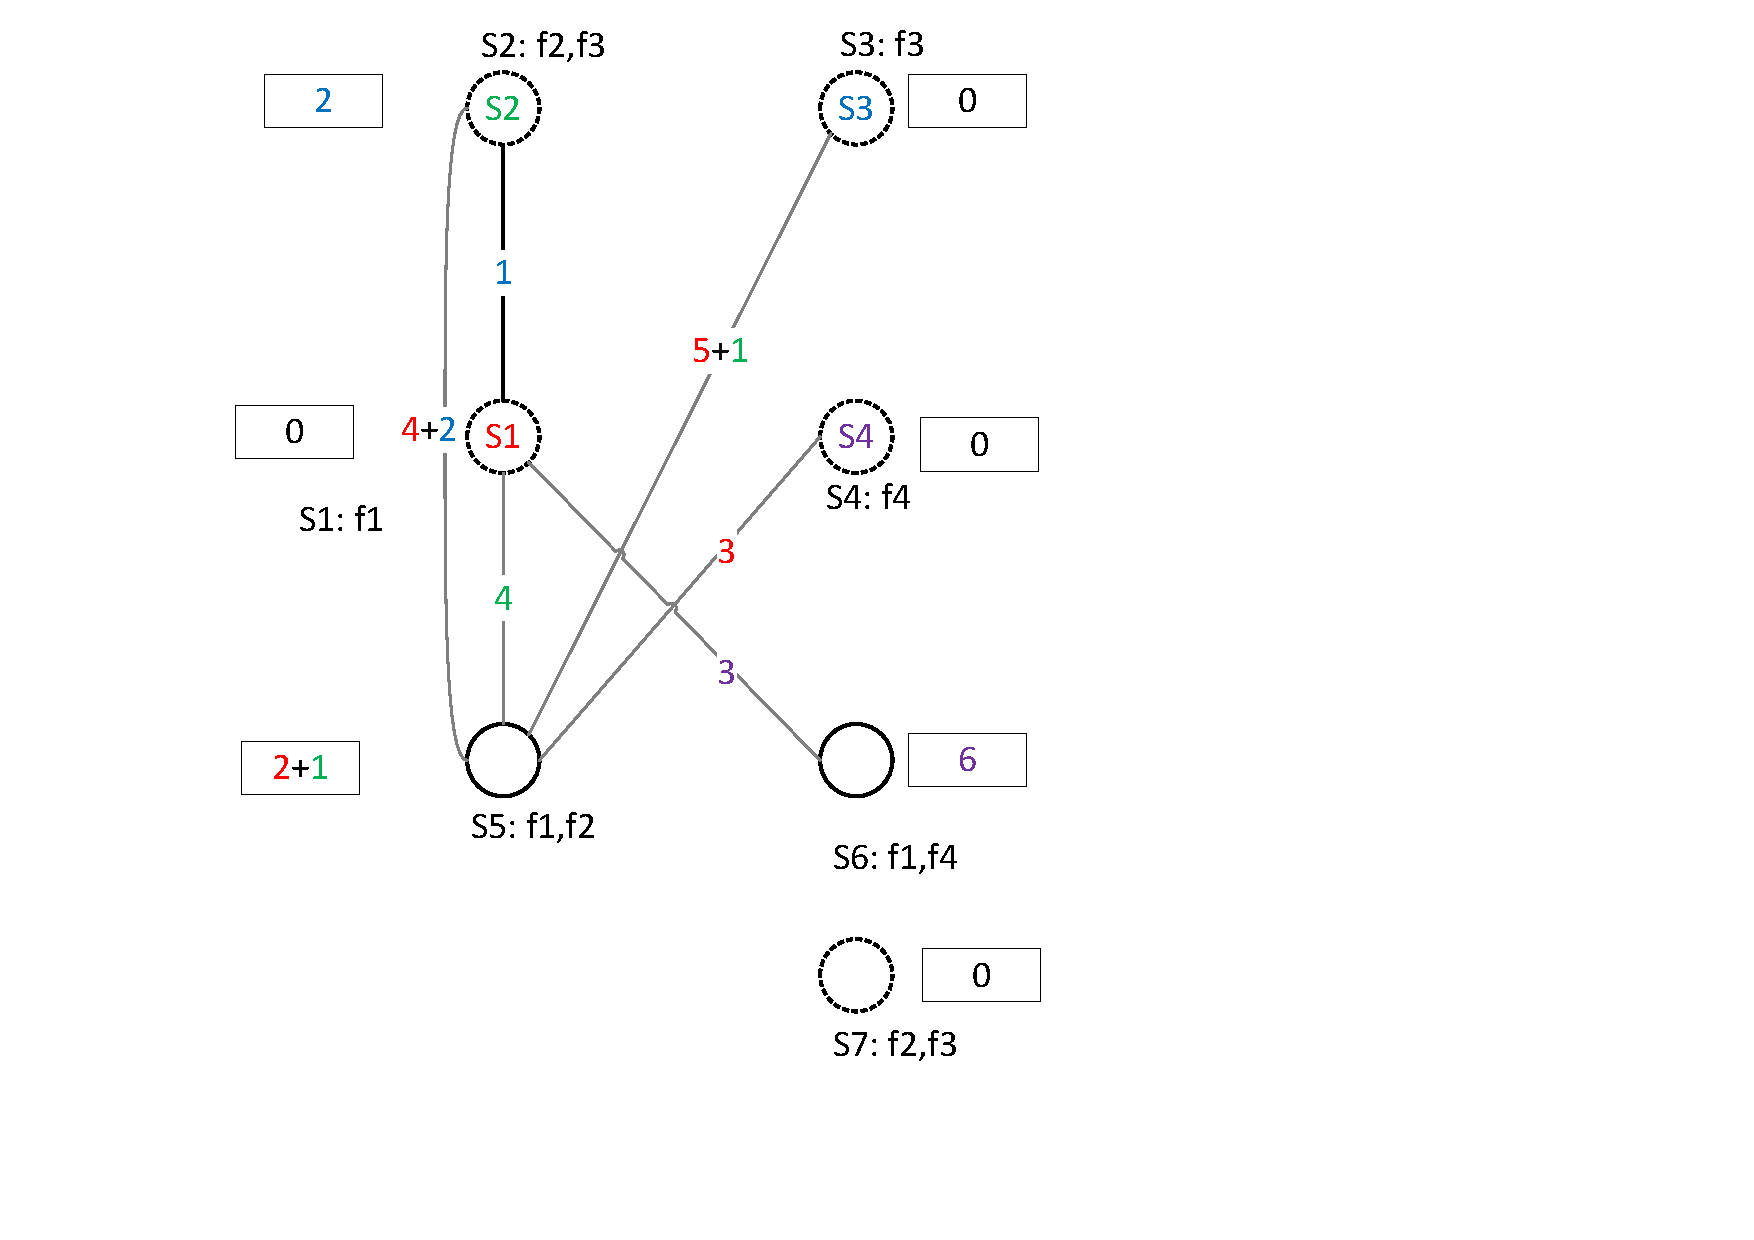
\includegraphics[width=1.5in]{Fig/AugmentResource}\\
  \caption{Augmented Resource}\label{fig:AugmentResource}
\end{figure}



Finally, we repeat the procedure of graph decomposition and multiple knapsack problem for each following node failure to construct the final FD-SeVN. As shown in Fig.\ref{fig:FD}, partial augment of the SeVN for each node failure is presented. It is
worth noting that, every step of partial enhancement is based on the latest step.


